% Options for packages loaded elsewhere
% Options for packages loaded elsewhere
\PassOptionsToPackage{unicode}{hyperref}
\PassOptionsToPackage{hyphens}{url}
\PassOptionsToPackage{dvipsnames,svgnames,x11names}{xcolor}
%
\documentclass[
  letterpaper,
  DIV=11,
  numbers=noendperiod]{scrartcl}
\usepackage{xcolor}
\usepackage{amsmath,amssymb}
\setcounter{secnumdepth}{-\maxdimen} % remove section numbering
\usepackage{iftex}
\ifPDFTeX
  \usepackage[T1]{fontenc}
  \usepackage[utf8]{inputenc}
  \usepackage{textcomp} % provide euro and other symbols
\else % if luatex or xetex
  \usepackage{unicode-math} % this also loads fontspec
  \defaultfontfeatures{Scale=MatchLowercase}
  \defaultfontfeatures[\rmfamily]{Ligatures=TeX,Scale=1}
\fi
\usepackage{lmodern}
\ifPDFTeX\else
  % xetex/luatex font selection
\fi
% Use upquote if available, for straight quotes in verbatim environments
\IfFileExists{upquote.sty}{\usepackage{upquote}}{}
\IfFileExists{microtype.sty}{% use microtype if available
  \usepackage[]{microtype}
  \UseMicrotypeSet[protrusion]{basicmath} % disable protrusion for tt fonts
}{}
\makeatletter
\@ifundefined{KOMAClassName}{% if non-KOMA class
  \IfFileExists{parskip.sty}{%
    \usepackage{parskip}
  }{% else
    \setlength{\parindent}{0pt}
    \setlength{\parskip}{6pt plus 2pt minus 1pt}}
}{% if KOMA class
  \KOMAoptions{parskip=half}}
\makeatother
% Make \paragraph and \subparagraph free-standing
\makeatletter
\ifx\paragraph\undefined\else
  \let\oldparagraph\paragraph
  \renewcommand{\paragraph}{
    \@ifstar
      \xxxParagraphStar
      \xxxParagraphNoStar
  }
  \newcommand{\xxxParagraphStar}[1]{\oldparagraph*{#1}\mbox{}}
  \newcommand{\xxxParagraphNoStar}[1]{\oldparagraph{#1}\mbox{}}
\fi
\ifx\subparagraph\undefined\else
  \let\oldsubparagraph\subparagraph
  \renewcommand{\subparagraph}{
    \@ifstar
      \xxxSubParagraphStar
      \xxxSubParagraphNoStar
  }
  \newcommand{\xxxSubParagraphStar}[1]{\oldsubparagraph*{#1}\mbox{}}
  \newcommand{\xxxSubParagraphNoStar}[1]{\oldsubparagraph{#1}\mbox{}}
\fi
\makeatother


\usepackage{longtable,booktabs,array}
\usepackage{calc} % for calculating minipage widths
% Correct order of tables after \paragraph or \subparagraph
\usepackage{etoolbox}
\makeatletter
\patchcmd\longtable{\par}{\if@noskipsec\mbox{}\fi\par}{}{}
\makeatother
% Allow footnotes in longtable head/foot
\IfFileExists{footnotehyper.sty}{\usepackage{footnotehyper}}{\usepackage{footnote}}
\makesavenoteenv{longtable}
\usepackage{graphicx}
\makeatletter
\newsavebox\pandoc@box
\newcommand*\pandocbounded[1]{% scales image to fit in text height/width
  \sbox\pandoc@box{#1}%
  \Gscale@div\@tempa{\textheight}{\dimexpr\ht\pandoc@box+\dp\pandoc@box\relax}%
  \Gscale@div\@tempb{\linewidth}{\wd\pandoc@box}%
  \ifdim\@tempb\p@<\@tempa\p@\let\@tempa\@tempb\fi% select the smaller of both
  \ifdim\@tempa\p@<\p@\scalebox{\@tempa}{\usebox\pandoc@box}%
  \else\usebox{\pandoc@box}%
  \fi%
}
% Set default figure placement to htbp
\def\fps@figure{htbp}
\makeatother





\setlength{\emergencystretch}{3em} % prevent overfull lines

\providecommand{\tightlist}{%
  \setlength{\itemsep}{0pt}\setlength{\parskip}{0pt}}



 


\KOMAoption{captions}{tableheading}
\makeatletter
\@ifpackageloaded{caption}{}{\usepackage{caption}}
\AtBeginDocument{%
\ifdefined\contentsname
  \renewcommand*\contentsname{Contents}
\else
  \newcommand\contentsname{Contents}
\fi
\ifdefined\listfigurename
  \renewcommand*\listfigurename{List of Figures}
\else
  \newcommand\listfigurename{List of Figures}
\fi
\ifdefined\listtablename
  \renewcommand*\listtablename{List of Tables}
\else
  \newcommand\listtablename{List of Tables}
\fi
\ifdefined\figurename
  \renewcommand*\figurename{Figure}
\else
  \newcommand\figurename{Figure}
\fi
\ifdefined\tablename
  \renewcommand*\tablename{Table}
\else
  \newcommand\tablename{Table}
\fi
}
\@ifpackageloaded{float}{}{\usepackage{float}}
\floatstyle{ruled}
\@ifundefined{c@chapter}{\newfloat{codelisting}{h}{lop}}{\newfloat{codelisting}{h}{lop}[chapter]}
\floatname{codelisting}{Listing}
\newcommand*\listoflistings{\listof{codelisting}{List of Listings}}
\makeatother
\makeatletter
\makeatother
\makeatletter
\@ifpackageloaded{caption}{}{\usepackage{caption}}
\@ifpackageloaded{subcaption}{}{\usepackage{subcaption}}
\makeatother
\usepackage{bookmark}
\IfFileExists{xurl.sty}{\usepackage{xurl}}{} % add URL line breaks if available
\urlstyle{same}
\hypersetup{
  pdftitle={Core Concepts of AI/ML for Earth Observation},
  pdfauthor={Stylianos Kotsopoulos},
  colorlinks=true,
  linkcolor={blue},
  filecolor={Maroon},
  citecolor={Blue},
  urlcolor={Blue},
  pdfcreator={LaTeX via pandoc}}


\title{Core Concepts of AI/ML for Earth Observation}
\usepackage{etoolbox}
\makeatletter
\providecommand{\subtitle}[1]{% add subtitle to \maketitle
  \apptocmd{\@title}{\par {\large #1 \par}}{}{}
}
\makeatother
\subtitle{CoPhil EO AI/ML Training - Day 1, Session 2}
\author{Stylianos Kotsopoulos}
\date{}
\begin{document}
\maketitle


\section{Welcome to Session 2}\label{welcome-to-session-2}

\subsection{Session Objectives}\label{session-objectives}

\begin{itemize}
\tightlist
\item
  Understand \textbf{what AI/ML means} in Earth Observation context
\item
  Learn the \textbf{end-to-end workflow} for ML projects
\item
  Distinguish \textbf{supervised} vs \textbf{unsupervised} learning
\item
  Grasp \textbf{deep learning} and neural network basics
\item
  Explore \textbf{2025 AI innovations} (foundation models, data-centric
  AI)
\end{itemize}

\textbf{Duration:} 2 hours

This session covers fundamental AI/ML concepts tailored to EO
applications. Mostly conceptual, but essential foundation for hands-on
work in Sessions 3-4 and throughout Day 2-4.

\begin{center}\rule{0.5\linewidth}{0.5pt}\end{center}

\subsection{Session Roadmap}\label{session-roadmap}

\begin{longtable}[]{@{}lll@{}}
\toprule\noalign{}
Time & Topic & Duration \\
\midrule\noalign{}
\endhead
\bottomrule\noalign{}
\endlastfoot
00-10 min & What is AI/ML? & 10 min \\
10-35 min & EO Workflow \& Data Pipeline & 25 min \\
35-60 min & Supervised vs Unsupervised Learning & 25 min \\
\textbf{60-65 min} & \textbf{☕ Break} & \textbf{5 min} \\
65-90 min & Deep Learning \& Neural Networks & 25 min \\
90-110 min & Data-Centric AI \& 2025 Updates & 20 min \\
110-120 min & Q\&A \& Summary & 10 min \\
\end{longtable}

\textbf{Timing:} 2 minutes

This session is more conceptual than Session 1. Focus on building
intuition and mental models. Hands-on practice comes in Sessions 3-4 and
Days 2-4.

\subsection{Why AI/ML for Earth
Observation?}\label{why-aiml-for-earth-observation}

\textbf{Traditional Approach}

\begin{itemize}
\tightlist
\item
  Manual interpretation
\item
  Rule-based classification
\item
  Simple thresholds
\item
  Time-consuming
\item
  Hard to scale
\end{itemize}

\textbf{AI/ML Approach}

\begin{itemize}
\tightlist
\item
  Automated pattern recognition
\item
  Learn from examples
\item
  Complex decision boundaries
\item
  Fast processing
\item
  Scalable to large areas
\end{itemize}

\textbf{ML can process years of satellite data in hours!}

Machine learning allows us to automatically recognize patterns in
satellite imagery without hard-coding rules for every scenario. This is
transformative for large-area, time-series analysis.

\section{What is AI/ML?}\label{what-is-aiml}

\subsection{Defining the Terms}\label{defining-the-terms}

\begin{figure}[H]

{\centering 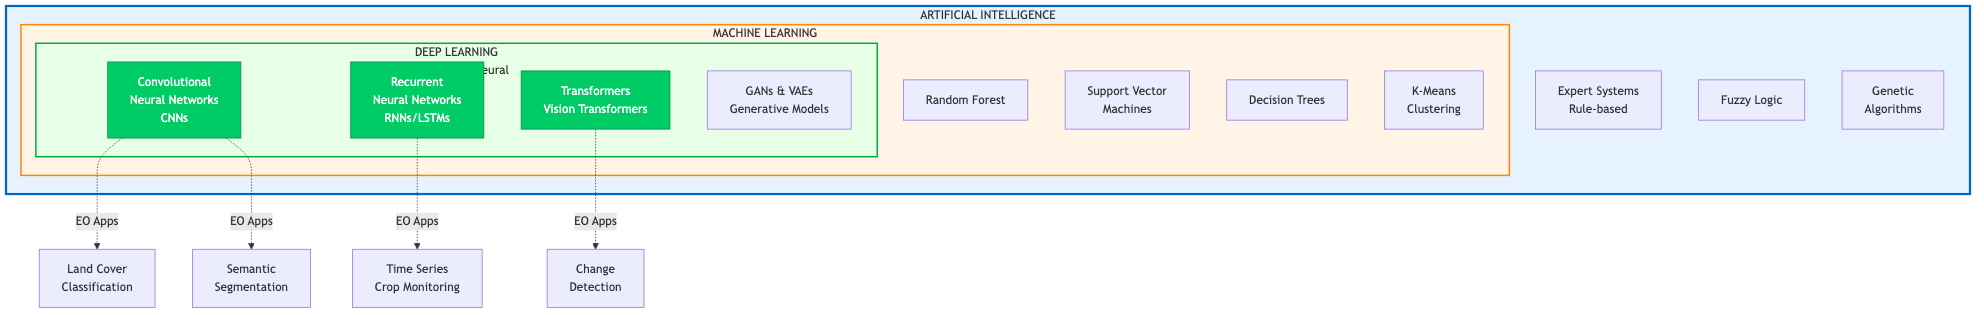
\includegraphics[width=0.85\linewidth,height=\textheight,keepaspectratio]{../../diagrams_export/diagram_006_day1_sessions_session2_1.png}

}

\caption{AI, ML, and Deep Learning Hierarchy with EO Applications}

\end{figure}%

\begin{itemize}
\tightlist
\item
  \textbf{Artificial Intelligence (AI):} Broad field of making machines
  ``smart''
\item
  \textbf{Machine Learning (ML):} Subset of AI where algorithms learn
  from data
\item
  \textbf{Deep Learning (DL):} Subset of ML using neural networks with
  many layers
\end{itemize}

AI is the broadest term. Machine Learning is a subset where computer
algorithms learn patterns from data without being explicitly programmed.
Deep Learning uses neural networks. This comprehensive diagram shows the
nested hierarchy with specific algorithms at each level (Random Forest,
CNNs, RNNs, etc.) and their Earth Observation applications like land
cover classification and time series analysis.

\subsection{Machine Learning in Simple
Terms}\label{machine-learning-in-simple-terms}

\textbf{Traditional Programming}

\begin{verbatim}
Rules + Data → Results
\end{verbatim}

\begin{itemize}
\tightlist
\item
  Programmer writes explicit rules
\item
  Fixed logic
\item
  Hard to handle complexity
\end{itemize}

\textbf{Machine Learning}

\begin{verbatim}
Data + Results → Rules
\end{verbatim}

\begin{itemize}
\tightlist
\item
  Algorithm learns rules from examples
\item
  Adaptive
\item
  Handles complex patterns
\end{itemize}

In traditional programming, we tell computers what to do step-by-step.
In ML, we show examples and the algorithm figures out the pattern.

\subsection{ML in Earth Observation
Context}\label{ml-in-earth-observation-context}

\textbf{Example: Forest vs Non-Forest}

\textbf{Traditional:}

\begin{verbatim}
IF NDVI > 0.6 THEN Forest
ELSE Non-Forest
\end{verbatim}

Simple, but breaks easily

\textbf{Machine Learning:}

\begin{itemize}
\tightlist
\item
  Show 1000 examples of forest pixels
\item
  Show 1000 examples of non-forest
\item
  Algorithm learns complex patterns
\item
  Works in diverse conditions
\end{itemize}

\begin{center}
\includegraphics[width=0.6\linewidth,height=\textheight,keepaspectratio]{images/classification_example.jpg}
\end{center}

A simple NDVI threshold might work in one region but fail in another. ML
can learn the nuanced patterns that distinguish forest from non-forest
across different conditions.

\section{The AI/ML Workflow for EO}\label{the-aiml-workflow-for-eo}

\subsection{End-to-End ML Workflow}\label{end-to-end-ml-workflow}

\begin{center}
\includegraphics[width=0.9\linewidth,height=\textheight,keepaspectratio]{images/ml_workflow.png}
\end{center}

This is the typical workflow for any ML project in Earth Observation.
Understanding these steps is crucial for successful implementation.

\subsection{Step 1: Problem Definition}\label{step-1-problem-definition}

\textbf{Key Questions}

\begin{itemize}
\tightlist
\item
  What exactly are we trying to achieve?
\item
  What decisions will this support?
\item
  What level of accuracy is needed?
\item
  What resources are available?
\end{itemize}

\textbf{EO Examples}

\begin{itemize}
\tightlist
\item
  Map rice paddy extent
\item
  Detect flooded areas after typhoon
\item
  Classify land cover types
\item
  Estimate crop yield
\item
  Monitor deforestation
\end{itemize}

\textbf{Clear problem definition = 50\% of success}

Being clear on the question helps design the solution. ``We want to
classify land cover in Palawan'' is much more actionable than ``We want
to use AI.''

\subsection{Step 2: Data Acquisition}\label{step-2-data-acquisition}

\textbf{Satellite Imagery}

\begin{itemize}
\tightlist
\item
  Sentinel-1/2 (covered in Session 1!)
\item
  Landsat
\item
  Planet
\item
  High-resolution commercial
\item
  Multiple dates/seasons
\end{itemize}

\textbf{Ground Truth / Labels}

\begin{itemize}
\tightlist
\item
  Field surveys
\item
  GPS points
\item
  Existing maps
\item
  Photo interpretation
\item
  Expert knowledge
\end{itemize}

\textbf{Challenge:} Getting quality labels is often hardest part

Data acquisition includes both satellite images and the ground truth
labels needed to train supervised models. The quality and quantity of
labels directly impact model performance.

\subsection{Step 3: Data Preprocessing}\label{step-3-data-preprocessing}

\textbf{For Satellite Imagery:}

\begin{itemize}
\tightlist
\item
  Atmospheric correction (use Level-2A!)
\item
  Cloud masking
\item
  Geometric correction
\item
  Radiometric calibration
\item
  Co-registration (multiple sensors)
\item
  Temporal compositing
\end{itemize}

\textbf{``Garbage In, Garbage Out''} - preprocessing matters!

Well-prepared input data is crucial. Even the best model will fail if
fed cloudy, misaligned, or uncorrected images.

\subsection{Preprocessing Example}\label{preprocessing-example}

\begin{figure}[H]

{\centering \includegraphics[width=0.9\linewidth,height=\textheight,keepaspectratio]{images/Cloud_removal_before_after.webp}

}

\caption{Cloud Removal Before and After Comparison}

\end{figure}%

\textbf{Before Preprocessing:} - Clouds present - Atmospheric haze -
Different acquisition dates

\textbf{After Preprocessing:} - Clouds masked - Atmospherically
corrected - Temporal composite created

Preprocessing transforms raw satellite data into analysis-ready
products. This side-by-side comparison shows the dramatic improvement
from cloud masking and creating temporal composites - essential steps
before any ML analysis.

\subsection{Step 4: Feature
Engineering}\label{step-4-feature-engineering}

\textbf{What are Features?}

\begin{itemize}
\tightlist
\item
  Input variables for the model
\item
  Derived from raw data
\item
  Informative for the task
\end{itemize}

\textbf{EO Features}

\begin{itemize}
\tightlist
\item
  Spectral bands (Blue, Red, NIR, etc.)
\item
  Spectral indices (NDVI, NDWI)
\item
  Texture measures
\item
  Temporal statistics
\item
  Topography (elevation, slope)
\end{itemize}

\textbf{Deep Learning:} Often learns features automatically!

For traditional ML like Random Forest, we engineer features. For deep
learning, the network learns features automatically from raw pixels.

\subsection{Common EO Features}\label{common-eo-features}

\begin{longtable}[]{@{}
  >{\raggedright\arraybackslash}p{(\linewidth - 4\tabcolsep) * \real{0.3214}}
  >{\raggedright\arraybackslash}p{(\linewidth - 4\tabcolsep) * \real{0.2500}}
  >{\raggedright\arraybackslash}p{(\linewidth - 4\tabcolsep) * \real{0.4286}}@{}}
\toprule\noalign{}
\begin{minipage}[b]{\linewidth}\raggedright
\textbf{Feature Type}
\end{minipage} & \begin{minipage}[b]{\linewidth}\raggedright
\textbf{Examples}
\end{minipage} & \begin{minipage}[b]{\linewidth}\raggedright
\textbf{What They Capture}
\end{minipage} \\
\midrule\noalign{}
\endhead
\bottomrule\noalign{}
\endlastfoot
\textbf{Spectral Bands} & B2, B3, B4, B8 & Reflectance at different
wavelengths \\
\textbf{Vegetation Indices} & NDVI, EVI, SAVI & Vegetation health,
density \\
\textbf{Water Indices} & NDWI, MNDWI & Water presence, moisture \\
\textbf{Texture} & GLCM variance, entropy & Spatial patterns \\
\textbf{Temporal} & Mean, std over time & Phenology, seasonality \\
\textbf{Topographic} & Elevation, slope, aspect & Terrain
characteristics \\
\end{longtable}

Different features highlight different aspects of the landscape.
Vegetation indices emphasize green biomass, water indices highlight
water bodies, etc.

\subsection{Step 5: Model Selection \&
Training}\label{step-5-model-selection-training}

\textbf{Model Selection}

Choose based on:

\begin{itemize}
\tightlist
\item
  Problem type (classification vs regression)
\item
  Data size
\item
  Interpretability needs
\item
  Computational resources
\end{itemize}

\textbf{Common EO Models}

\begin{itemize}
\tightlist
\item
  Random Forest
\item
  Support Vector Machines
\item
  Convolutional Neural Networks
\item
  U-Net (segmentation)
\item
  Recurrent networks (time series)
\end{itemize}

Model choice depends on your specific problem, available data, and
resources. We'll cover Random Forest on Day 2 and CNNs on Day 3.

\subsection{Training Process}\label{training-process}

\begin{center}
\includegraphics[width=0.75\linewidth,height=\textheight,keepaspectratio]{images/training_process.png}
\end{center}

\begin{enumerate}
\def\labelenumi{\arabic{enumi}.}
\tightlist
\item
  \textbf{Split data:} Training set (70-80\%) \& Validation set
  (20-30\%)
\item
  \textbf{Feed training data} to model
\item
  \textbf{Model learns patterns} by adjusting internal parameters
\item
  \textbf{Validate} on unseen validation data
\item
  \textbf{Iterate:} Adjust model or data if needed
\end{enumerate}

Training involves feeding labeled examples to the model. The model
adjusts its internal parameters to minimize errors on the training data.

\subsection{Step 6: Validation \&
Evaluation}\label{step-6-validation-evaluation}

\textbf{Why Validate?}

\begin{itemize}
\tightlist
\item
  Ensure model generalizes
\item
  Detect overfitting
\item
  Compare different models
\item
  Build confidence
\end{itemize}

\textbf{Evaluation Metrics}

\begin{itemize}
\tightlist
\item
  Overall Accuracy
\item
  Confusion Matrix
\item
  Precision \& Recall
\item
  F1-Score
\item
  Kappa coefficient
\end{itemize}

\textbf{Use independent test data - never validate on training data!}

Rigorous validation using held-out data ensures the model works on new,
unseen examples - not just memorizing training data.

\subsection{Confusion Matrix Example}\label{confusion-matrix-example}

\begin{center}
\includegraphics[width=0.6\linewidth,height=\textheight,keepaspectratio]{images/confusion_matrix.png}
\end{center}

\textbf{What it shows:}

\begin{itemize}
\tightlist
\item
  True Positives (correct predictions)
\item
  False Positives (type I error)
\item
  False Negatives (type II error)
\item
  True Negatives
\end{itemize}

\textbf{Derived Metrics:}

\begin{itemize}
\tightlist
\item
  Precision = TP / (TP + FP)
\item
  Recall = TP / (TP + FN)
\item
  Accuracy = (TP + TN) / Total
\end{itemize}

The confusion matrix shows where your model is making mistakes. This
helps identify which classes are being confused.

\subsection{Step 7: Deployment}\label{step-7-deployment}

\textbf{Deployment Options}

\begin{itemize}
\tightlist
\item
  Generate full maps
\item
  Near real-time monitoring
\item
  Operational pipelines
\item
  Decision support systems
\item
  Web applications
\end{itemize}

\textbf{Considerations}

\begin{itemize}
\tightlist
\item
  Model retraining schedule
\item
  Computational requirements
\item
  User interface
\item
  Data updates
\item
  Maintenance plan
\end{itemize}

If the model is satisfactory, deploy it for operational use. This might
mean generating maps for entire regions or setting up automatic
processing of new satellite images.

\subsection{Workflow is Iterative}\label{workflow-is-iterative}

\begin{center}
\includegraphics[width=0.7\linewidth,height=\textheight,keepaspectratio]{images/iterative_workflow.png}
\end{center}

\begin{itemize}
\tightlist
\item
  \textbf{Poor validation?} → Go back to data acquisition or model
  selection
\item
  \textbf{New data available?} → Retrain model
\item
  \textbf{Requirements change?} → Redefine problem
\item
  \textbf{Continuous improvement} is key
\end{itemize}

Real projects are iterative. You often loop back: if validation is poor,
you might need more data, different features, or a different model.

\section{Types of Machine Learning}\label{types-of-machine-learning}

\subsection{Main ML Paradigms}\label{main-ml-paradigms}

\begin{center}
\includegraphics[width=0.75\linewidth,height=\textheight,keepaspectratio]{images/ml_types.png}
\end{center}

\begin{enumerate}
\def\labelenumi{\arabic{enumi}.}
\tightlist
\item
  \textbf{Supervised Learning} (most common in EO)
\item
  \textbf{Unsupervised Learning} (exploratory analysis)
\item
  \textbf{Semi-supervised Learning} (combines both)
\item
  \textbf{Reinforcement Learning} (less common in EO)
\end{enumerate}

We'll focus on supervised and unsupervised learning as these are most
relevant for Earth Observation applications.

\section{Supervised Learning}\label{supervised-learning}

\subsection{What is Supervised
Learning?}\label{what-is-supervised-learning}

\textbf{Definition}

\begin{itemize}
\tightlist
\item
  Learning from \textbf{labeled data}
\item
  Known input-output pairs
\item
  Model learns mapping from inputs to outputs
\item
  Like learning with an answer key
\end{itemize}

\includegraphics[width=1\linewidth,height=\textheight,keepaspectratio]{images/supervised_learning.png}

\textbf{Requires ground truth labels for training}

Supervised learning is the most common in EO. The algorithm is given
examples with known outcomes (labels) and learns to predict labels for
new, unseen data.

\subsection{Two Types of Supervised
Learning}\label{two-types-of-supervised-learning}

\textbf{Classification}

\begin{itemize}
\tightlist
\item
  Predict \textbf{categorical} labels
\item
  Discrete classes
\item
  Example outputs: ``Forest'', ``Water'', ``Urban''
\end{itemize}

\includegraphics[width=1\linewidth,height=\textheight,keepaspectratio]{images/classification.jpg}

\textbf{Regression}

\begin{itemize}
\tightlist
\item
  Predict \textbf{continuous} values
\item
  Numeric outputs
\item
  Example outputs: 25.3 tons/hectare, 15.2°C
\end{itemize}

\includegraphics[width=1\linewidth,height=\textheight,keepaspectratio]{images/regression.jpg}

Classification assigns data to categories. Regression predicts numeric
values. Both require labeled training data.

\subsection{Classification Examples in
EO}\label{classification-examples-in-eo}

\textbf{Land Cover Classification}

\includegraphics[width=1\linewidth,height=\textheight,keepaspectratio]{images/land_cover_classification.jpg}

\begin{itemize}
\tightlist
\item
  Forest, agriculture, urban, water
\item
  Pixel-wise or object-based
\item
  Multi-class problem
\end{itemize}

\textbf{Crop Type Mapping}

\includegraphics[width=1\linewidth,height=\textheight,keepaspectratio]{images/crop_type_map.jpg}

\begin{itemize}
\tightlist
\item
  Rice, corn, sugarcane
\item
  Seasonal patterns important
\item
  Supports agricultural planning
\end{itemize}

Land cover classification is the classic EO supervised learning task.
Each pixel or region is assigned to a class like forest, water, or
urban.

\subsection{Regression Examples in EO}\label{regression-examples-in-eo}

\textbf{Biomass Estimation}

\includegraphics[width=1\linewidth,height=\textheight,keepaspectratio]{images/biomass_estimation.jpg}

\begin{itemize}
\tightlist
\item
  Predict tons of biomass per hectare
\item
  Important for carbon accounting
\item
  Uses SAR and optical data
\end{itemize}

\textbf{Crop Yield Prediction}

\includegraphics[width=1\linewidth,height=\textheight,keepaspectratio]{images/yield_prediction.jpg}

\begin{itemize}
\tightlist
\item
  Predict tons per hectare
\item
  Seasonal NDVI time series
\item
  Supports food security planning
\end{itemize}

Regression tasks predict continuous values like biomass density, crop
yield, soil moisture, or sea surface temperature from satellite data.

\subsection{Common Supervised
Algorithms}\label{common-supervised-algorithms}

\begin{longtable}[]{@{}
  >{\raggedright\arraybackslash}p{(\linewidth - 4\tabcolsep) * \real{0.2941}}
  >{\raggedright\arraybackslash}p{(\linewidth - 4\tabcolsep) * \real{0.2941}}
  >{\raggedright\arraybackslash}p{(\linewidth - 4\tabcolsep) * \real{0.4118}}@{}}
\toprule\noalign{}
\begin{minipage}[b]{\linewidth}\raggedright
\textbf{Algorithm}
\end{minipage} & \begin{minipage}[b]{\linewidth}\raggedright
\textbf{Strengths}
\end{minipage} & \begin{minipage}[b]{\linewidth}\raggedright
\textbf{EO Applications}
\end{minipage} \\
\midrule\noalign{}
\endhead
\bottomrule\noalign{}
\endlastfoot
\textbf{Random Forest} & Handles high dimensions, robust & Land cover,
crop classification \\
\textbf{SVM} & Effective in high dimensions & Binary classification,
change detection \\
\textbf{Neural Networks} & Learns complex patterns & Image
classification, segmentation \\
\textbf{Decision Trees} & Interpretable & Quick classifications \\
\textbf{k-NN} & Simple, non-parametric & Local classifications \\
\end{longtable}

Different algorithms have different strengths. Random Forest is popular
in EO for its robustness and ability to handle many features.

\subsection{Supervised Learning
Requirements}\label{supervised-learning-requirements}

\textbf{Essential:}

\begin{enumerate}
\def\labelenumi{\arabic{enumi}.}
\tightlist
\item
  \textbf{Training data} with known labels
\item
  \textbf{Representative samples} covering all classes
\item
  \textbf{Sufficient quantity} (varies by algorithm)
\item
  \textbf{Quality labels} (accurate, consistent)
\item
  \textbf{Independent validation} data
\end{enumerate}

\textbf{Challenge:} Getting quality labels is often the bottleneck!

Supervised learning needs ground truth. For land cover, this might be
field surveys, GPS points, or careful photo interpretation. Quality
matters more than quantity!

\section{Unsupervised Learning}\label{unsupervised-learning}

\subsection{What is Unsupervised
Learning?}\label{what-is-unsupervised-learning}

\textbf{Definition}

\begin{itemize}
\tightlist
\item
  Learning from \textbf{unlabeled data}
\item
  No known outputs
\item
  Discover hidden patterns
\item
  Like sorting without instructions
\end{itemize}

\includegraphics[width=1\linewidth,height=\textheight,keepaspectratio]{images/unsupervised_learning.png}

\textbf{Useful for exploratory analysis and finding structure}

Unsupervised learning finds patterns or groupings inherent in the data
without being told what to look for.

\subsection{Clustering: Main Unsupervised
Technique}\label{clustering-main-unsupervised-technique}

\begin{center}
\includegraphics[width=0.7\linewidth,height=\textheight,keepaspectratio]{images/clustering_example.png}
\end{center}

\begin{itemize}
\tightlist
\item
  \textbf{Group similar pixels} based on spectral characteristics
\item
  Algorithm decides number of clusters (or you specify)
\item
  \textbf{Analyst interprets} what each cluster means
\item
  Example: ``Cluster 3 looks like water, Cluster 7 looks like forest''
\end{itemize}

K-means clustering is a common unsupervised method. It groups pixels
with similar reflectance, but you have to interpret what those groups
mean.

\subsection{Unsupervised EO
Applications}\label{unsupervised-eo-applications}

\textbf{Change Detection}

\begin{itemize}
\tightlist
\item
  Cluster ``before'' and ``after'' images
\item
  Identify changed areas
\item
  No labels needed
\end{itemize}

\textbf{Anomaly Detection}

\begin{itemize}
\tightlist
\item
  Find unusual pixels
\item
  Potential forest disturbance
\item
  Data quality issues
\end{itemize}

\textbf{Initial Exploration}

\begin{itemize}
\tightlist
\item
  Quick overview of spectral classes
\item
  Inform supervised approach
\item
  Generate training samples
\end{itemize}

\textbf{Dimensionality Reduction}

\begin{itemize}
\tightlist
\item
  PCA, t-SNE
\item
  Visualize high-dimensional data
\item
  Feature extraction
\end{itemize}

Unsupervised methods are useful for quick initial analysis or when you
don't have ground truth labels. Results need interpretation though.

\subsection{Supervised vs
Unsupervised}\label{supervised-vs-unsupervised}

\begin{longtable}[]{@{}
  >{\raggedright\arraybackslash}p{(\linewidth - 4\tabcolsep) * \real{0.2609}}
  >{\raggedright\arraybackslash}p{(\linewidth - 4\tabcolsep) * \real{0.3478}}
  >{\raggedright\arraybackslash}p{(\linewidth - 4\tabcolsep) * \real{0.3913}}@{}}
\toprule\noalign{}
\begin{minipage}[b]{\linewidth}\raggedright
\textbf{Aspect}
\end{minipage} & \begin{minipage}[b]{\linewidth}\raggedright
\textbf{Supervised}
\end{minipage} & \begin{minipage}[b]{\linewidth}\raggedright
\textbf{Unsupervised}
\end{minipage} \\
\midrule\noalign{}
\endhead
\bottomrule\noalign{}
\endlastfoot
\textbf{Labels} & Required & Not needed \\
\textbf{Accuracy} & Generally higher & Lower, needs interpretation \\
\textbf{Use Case} & Precise classification & Exploration, pattern
discovery \\
\textbf{Effort} & High (collecting labels) & Low (no labels) \\
\textbf{Output} & Predefined classes & Discovered clusters \\
\textbf{Control} & High (you define classes) & Low (algorithm decides
groups) \\
\end{longtable}

Supervised methods generally yield more accurate results when good
training data is available. Unsupervised is useful when labels are
unavailable or for exploratory work.

\subsection{Which to Choose?}\label{which-to-choose}

\textbf{Use Supervised When:}

\begin{itemize}
\tightlist
\item
  You have ground truth labels
\item
  Need specific classes
\item
  Accuracy is critical
\item
  Operational application
\end{itemize}

\textbf{Use Unsupervised When:}

\begin{itemize}
\tightlist
\item
  No labels available
\item
  Exploratory analysis
\item
  Discovering unknown patterns
\item
  Quick initial assessment
\end{itemize}

\textbf{In practice:} Often combine both approaches!

Most operational EO applications use supervised learning because
accuracy and specific class definitions are important. Unsupervised
helps with initial exploration.

\begin{center}\rule{0.5\linewidth}{0.5pt}\end{center}

\subsection{☕ 5-Minute Break}\label{minute-break}

\textbf{Stretch Break}

Stand up • Grab water • Back in 5 minutes

\textbf{Timing:} 5 minutes

\textbf{Instructor Actions:} - Announce break - Mention we'll dive into
deep learning next - Be available for quick questions

\textbf{When Resuming:} - Quick recap: ``We've covered ML basics,
workflow, supervised/unsupervised. Now: deep learning!''

\begin{center}\rule{0.5\linewidth}{0.5pt}\end{center}

\section{Introduction to Deep
Learning}\label{introduction-to-deep-learning}

\subsection{What is Deep Learning?}\label{what-is-deep-learning}

\textbf{Deep Learning = Neural Networks with Many Layers}

\begin{itemize}
\tightlist
\item
  Subset of machine learning
\item
  ``Deep'' refers to multiple layers
\item
  Automatically learns features
\item
  Excels at image analysis
\item
  Data-hungry
\end{itemize}

\includegraphics[width=1\linewidth,height=\textheight,keepaspectratio]{images/deep_learning_layers.png}

Deep learning is essentially about neural networks with many layers
(dozens or even hundreds). These ``deep'' networks can capture very
complex relationships.

\subsection{Neural Networks: Building
Blocks}\label{neural-networks-building-blocks}

\begin{center}
\includegraphics[width=0.7\linewidth,height=\textheight,keepaspectratio]{images/neuron_diagram.png}
\end{center}

\textbf{Artificial Neuron:}

\begin{enumerate}
\def\labelenumi{\arabic{enumi}.}
\tightlist
\item
  Takes multiple inputs
\item
  Multiplies each by a \textbf{weight}
\item
  Adds a \textbf{bias}
\item
  Applies \textbf{activation function}
\item
  Produces output
\end{enumerate}

A single neuron is like a logistic regression unit. It takes inputs,
applies weights, and uses an activation function to produce an output.

\subsection{Neural Network
Architecture}\label{neural-network-architecture}

\begin{center}
\includegraphics[width=0.8\linewidth,height=\textheight,keepaspectratio]{images/neural_network_architecture.png}
\end{center}

\textbf{Layers:}

\begin{itemize}
\tightlist
\item
  \textbf{Input Layer:} Receives data (e.g., pixel values)
\item
  \textbf{Hidden Layers:} Process and transform
\item
  \textbf{Output Layer:} Final prediction
\end{itemize}

\textbf{Connections:}

\begin{itemize}
\tightlist
\item
  Each neuron connects to next layer
\item
  Weights on connections
\item
  Information flows forward
\end{itemize}

Neurons are organized into layers. The input layer receives data (pixel
values), hidden layers progressively extract features, and the output
layer makes predictions.

\subsection{Key Concepts}\label{key-concepts}

\textbf{Activation Functions}

\begin{itemize}
\tightlist
\item
  Introduce non-linearity
\item
  Common: ReLU, Sigmoid, Tanh
\item
  Allow network to learn complex patterns
\end{itemize}

\textbf{Weights and Biases}

\begin{itemize}
\tightlist
\item
  Parameters the network learns
\item
  Millions of parameters in deep networks
\item
  Adjusted during training
\end{itemize}

\textbf{Forward Propagation}

\begin{itemize}
\tightlist
\item
  Data flows input → output
\item
  Generate prediction
\end{itemize}

Activation functions are crucial - they allow neural networks to learn
non-linear relationships. Without them, the network would just be linear
regression!

\subsection{How Neural Networks Learn}\label{how-neural-networks-learn}

\begin{center}
\includegraphics[width=0.75\linewidth,height=\textheight,keepaspectratio]{images/training_loop.png}
\end{center}

\begin{enumerate}
\def\labelenumi{\arabic{enumi}.}
\tightlist
\item
  \textbf{Forward pass:} Input data, get prediction
\item
  \textbf{Calculate loss:} How wrong is the prediction?
\item
  \textbf{Backpropagation:} Calculate gradients
\item
  \textbf{Update weights:} Adjust to reduce error
\item
  \textbf{Repeat:} Thousands of times (epochs)
\end{enumerate}

Training adjusts weights to minimize error. This happens through
backpropagation - computing gradients and updating weights in the
direction that reduces loss.

\subsection{Loss Functions}\label{loss-functions}

\textbf{Classification}

\textbf{Cross-Entropy Loss}

\begin{itemize}
\tightlist
\item
  Measures classification error
\item
  Higher penalty for confident wrong predictions
\item
  Standard for multi-class problems
\end{itemize}

\textbf{Regression}

\textbf{Mean Squared Error}

\[MSE = \frac{1}{n}\sum_{i=1}^{n}(y_i - \hat{y}_i)^2\]

\begin{itemize}
\tightlist
\item
  Measures prediction error
\item
  Squared difference from true value
\end{itemize}

Loss functions quantify ``how bad'' predictions are. The training
process tries to minimize this loss by adjusting weights.

\subsection{Optimizers}\label{optimizers}

\textbf{Stochastic Gradient Descent (SGD)}

\begin{itemize}
\tightlist
\item
  Basic optimizer
\item
  Updates weights based on gradients
\item
  Learning rate controls step size
\end{itemize}

\textbf{Adam Optimizer}

\begin{itemize}
\tightlist
\item
  Adaptive learning rates
\item
  Faster convergence
\item
  Most popular for deep learning
\item
  Generally works well
\end{itemize}

\textbf{You don't need to implement these - frameworks do it for you!}

Optimizers determine how weights are updated. Adam is the most popular
because it adapts learning rates automatically and generally converges
faster than SGD.

\subsection{Convolutional Neural Networks
(CNNs)}\label{convolutional-neural-networks-cnns}

\begin{center}
\includegraphics[width=0.85\linewidth,height=\textheight,keepaspectratio]{images/cnn_architecture.png}
\end{center}

\textbf{Specialized for images:}

\begin{itemize}
\tightlist
\item
  \textbf{Convolutional layers:} Detect spatial patterns
\item
  \textbf{Pooling layers:} Reduce dimensionality
\item
  \textbf{Fully connected layers:} Final classification
\item
  Automatically learn features (edges, textures, objects)
\end{itemize}

CNNs are neural networks specialized for grid data like images. They use
convolutional layers to automatically extract spatial features.

\subsection{How CNNs Process Images}\label{how-cnns-process-images}

\begin{center}
\includegraphics[width=0.8\linewidth,height=\textheight,keepaspectratio]{images/cnn_feature_extraction.png}
\end{center}

\textbf{Hierarchical Feature Learning:}

\begin{itemize}
\tightlist
\item
  \textbf{Early layers:} Detect edges, simple patterns
\item
  \textbf{Middle layers:} Detect textures, parts
\item
  \textbf{Later layers:} Detect objects, scenes
\item
  \textbf{No manual feature engineering needed!}
\end{itemize}

CNNs learn increasingly complex features at each layer. Early layers
detect edges, later layers detect whole objects. This happens
automatically during training!

\subsection{CNNs in Earth Observation}\label{cnns-in-earth-observation}

\textbf{Applications:}

\begin{itemize}
\tightlist
\item
  Image classification
\item
  Object detection (ships, buildings)
\item
  Semantic segmentation (pixel-wise)
\item
  Change detection
\item
  Super-resolution
\end{itemize}

\textbf{Advantages:}

\begin{itemize}
\tightlist
\item
  Learn features automatically
\item
  Handle spatial context
\item
  State-of-the-art performance
\item
  Transfer learning possible
\end{itemize}

\begin{center}
\includegraphics[width=0.7\linewidth,height=\textheight,keepaspectratio]{images/cnn_eo_examples.jpg}
\end{center}

CNNs have achieved state-of-the-art results in many EO tasks. They can
learn to recognize complex patterns without manual feature engineering.

\subsection{Popular CNN Architectures for
EO}\label{popular-cnn-architectures-for-eo}

\begin{longtable}[]{@{}
  >{\raggedright\arraybackslash}p{(\linewidth - 6\tabcolsep) * \real{0.2769}}
  >{\raggedright\arraybackslash}p{(\linewidth - 6\tabcolsep) * \real{0.1538}}
  >{\raggedright\arraybackslash}p{(\linewidth - 6\tabcolsep) * \real{0.2923}}
  >{\raggedright\arraybackslash}p{(\linewidth - 6\tabcolsep) * \real{0.2769}}@{}}
\toprule\noalign{}
\begin{minipage}[b]{\linewidth}\raggedright
\textbf{Architecture}
\end{minipage} & \begin{minipage}[b]{\linewidth}\raggedright
\textbf{Year}
\end{minipage} & \begin{minipage}[b]{\linewidth}\raggedright
\textbf{Key Innovation}
\end{minipage} & \begin{minipage}[b]{\linewidth}\raggedright
\textbf{EO Use Cases}
\end{minipage} \\
\midrule\noalign{}
\endhead
\bottomrule\noalign{}
\endlastfoot
\textbf{ResNet} & 2015 & Residual connections & Classification, backbone
for detection \\
\textbf{U-Net} & 2015 & Skip connections & Semantic segmentation, flood
mapping \\
\textbf{EfficientNet} & 2019 & Compound scaling & Efficient
classification, mobile deployment \\
\textbf{DeepLabv3+} & 2018 & Atrous convolution & Land cover
segmentation \\
\textbf{YOLOv8} & 2023 & Real-time detection & Object detection,
ship/vehicle counting \\
\end{longtable}

\textbf{ResNet and EfficientNet are most popular backbones for EO}

These are proven architectures widely used in EO. ResNet-50 is often the
starting point for transfer learning. U-Net dominates semantic
segmentation tasks.

\subsection{ResNet: Residual Networks}\label{resnet-residual-networks}

\begin{center}
\includegraphics[width=0.7\linewidth,height=\textheight,keepaspectratio]{images/resnet_residual_block.png}
\end{center}

\textbf{Key Innovation: Skip Connections}

\begin{itemize}
\tightlist
\item
  Allows training very deep networks (50, 101, 152 layers)
\item
  Solves vanishing gradient problem
\item
  Identity mapping preserves information
\end{itemize}

\textbf{Common Variants:} - ResNet-50 (25M parameters) - ResNet-101 (44M
parameters) - ResNet-152 (60M parameters)

\textbf{EO Applications:}

\begin{itemize}
\tightlist
\item
  Pre-trained on ImageNet
\item
  Fine-tune for EO tasks
\item
  Backbone for object detection
\item
  Transfer learning baseline
\end{itemize}

\textbf{Performance:} - Top-5 error: 3.57\% (ImageNet) - Works well with
10k+ images

ResNet revolutionized deep learning by enabling training of very deep
networks. Skip connections allow gradients to flow directly through the
network.

\subsection{U-Net for Semantic
Segmentation}\label{u-net-for-semantic-segmentation}

\begin{center}
\includegraphics[width=0.8\linewidth,height=\textheight,keepaspectratio]{images/unet_architecture.png}
\end{center}

\textbf{Architecture:} - \textbf{Encoder (contracting path):} Captures
context - \textbf{Decoder (expanding path):} Enables precise
localization - \textbf{Skip connections:} Combine low \& high-level
features

\textbf{Why Dominant in EO:} - Works with small datasets (hundreds of
images) - Precise pixel-wise predictions - Perfect for segmentation
tasks

\textbf{EO Applications:} Flood mapping, land cover, building
footprints, crop fields

U-Net is THE architecture for semantic segmentation in EO. Originally
designed for biomedical image segmentation, it's now standard for
pixel-wise classification tasks.

\subsection{Deep Learning Frameworks}\label{deep-learning-frameworks}

\textbf{TensorFlow / Keras}

\includegraphics[width=1.5625in,height=\textheight,keepaspectratio]{images/tensorflow_logo.png}

\begin{itemize}
\tightlist
\item
  Google's framework
\item
  High-level Keras API
\item
  Production-ready
\item
  Large ecosystem
\end{itemize}

\textbf{PyTorch}

\includegraphics[width=1.5625in,height=\textheight,keepaspectratio]{images/pytorch_logo.png}

\begin{itemize}
\tightlist
\item
  Facebook's framework
\item
  Pythonic and intuitive
\item
  Popular in research
\item
  Flexible
\end{itemize}

\textbf{We'll use TensorFlow/Keras in this training}

You don't implement backpropagation yourself - frameworks like
TensorFlow and PyTorch handle the math. You just define the architecture
and provide data.

\subsection{Deep Learning
Considerations}\label{deep-learning-considerations}

\textbf{Advantages:}

\begin{itemize}
\tightlist
\item
  Automatic feature learning
\item
  State-of-the-art accuracy
\item
  Handles complex patterns
\item
  Scales to big data
\end{itemize}

\textbf{Challenges:}

\begin{itemize}
\tightlist
\item
  Requires lots of training data
\item
  Computationally intensive (need GPUs)
\item
  Less interpretable (``black box'')
\item
  Harder to debug
\end{itemize}

\textbf{Start simple (Random Forest), move to DL when you have data and
compute}

Deep learning is powerful but data-hungry and computationally expensive.
For many EO tasks, simpler models like Random Forest work well with less
data.

\section{Benchmark Datasets for EO}\label{benchmark-datasets-for-eo}

\subsection{Why Benchmark Datasets
Matter}\label{why-benchmark-datasets-matter}

\begin{enumerate}
\def\labelenumi{\arabic{enumi}.}
\tightlist
\item
  \textbf{Standardized Evaluation} - Compare algorithms objectively
\item
  \textbf{Training Resources} - Pre-labeled data for model training
\item
  \textbf{Transfer Learning} - Pre-train on large datasets, fine-tune
  locally
\item
  \textbf{Research Reproducibility} - Enable comparison across studies
\item
  \textbf{Community Building} - Shared resources accelerate progress
\end{enumerate}

\textbf{You don't need to label everything from scratch!}

Benchmark datasets are crucial for EO ML. They provide labeled training
data and enable fair comparison of methods across research groups
worldwide.

\subsection{EuroSAT: Land Cover
Classification}\label{eurosat-land-cover-classification}

\textbf{Specifications:} - \textbf{Images:} 27,000 labeled patches -
\textbf{Classes:} 10 land cover types - \textbf{Size:} 64×64 pixels -
\textbf{Bands:} All 13 Sentinel-2 bands - \textbf{Source:} European
cities

\textbf{10 Classes:} Annual Crop • Forest • Herbaceous Vegetation •
Highway • Industrial • Pasture • Permanent Crop • Residential • River •
Sea/Lake

\includegraphics[width=1\linewidth,height=\textheight,keepaspectratio]{images/eurosat_classes.png}

\textbf{Achievement:} \textbf{98.57\% accuracy} with CNNs

\textbf{Why Popular:} - Sentinel-2 based - Balanced classes - Easy to
use

EuroSAT is one of the most popular benchmarks for EO classification.
Based on Sentinel-2, making it highly relevant for operational
applications. Great starting point for CNN experiments.

\subsection{BigEarthNet: Large-Scale
Multi-Label}\label{bigearthnet-large-scale-multi-label}

\textbf{Massive Scale:} - \textbf{Images:} 590,326 Sentinel-2 patches -
\textbf{Coverage:} 10 European countries - \textbf{Labels:} 43 land
cover classes - \textbf{Multi-label:} Multiple classes per image -
\textbf{Multi-modal:} Optical + SAR version

\textbf{Real-World Complexity:} - Forest + Water - Urban + Agricultural
- Reflects actual landscapes

\includegraphics[width=1\linewidth,height=\textheight,keepaspectratio]{images/bigearth_multilabel.jpg}

\textbf{Why Different:}

Unlike EuroSAT (single label), BigEarthNet has multiple overlapping
classes - more realistic!

\textbf{Access:} - bigearth.net - TensorFlow Datasets - Papers With Code

BigEarthNet's multi-label nature makes it more challenging but also more
realistic. Essential for semantic segmentation research and testing
advanced architectures.

\subsection{xView: Object Detection
Benchmark}\label{xview-object-detection-benchmark}

\textbf{Specifications:} - \textbf{Objects:} \textgreater1 million
annotated - \textbf{Classes:} 60 object types - \textbf{Resolution:}
0.3m (WorldView-3) - \textbf{Area:} \textgreater1,400 km² -
\textbf{Annotations:} Bounding boxes

\textbf{Object Categories:} - Buildings \& infrastructure - Vehicles
(cars, trucks, aircraft) - Ships \& maritime - Storage tanks -
Construction equipment

\includegraphics[width=1\linewidth,height=\textheight,keepaspectratio]{images/xview_samples.jpg}

\textbf{Created for disaster response}

\textbf{Applications:} - YOLO training - Faster R-CNN - Small object
detection - Infrastructure mapping

xView is THE benchmark for object detection in satellite imagery.
Created for disaster response applications, now widely used for testing
detection algorithms like YOLO and Faster R-CNN.

\subsection{Philippine Data Resources}\label{philippine-data-resources}

\textbf{PRiSM (PhilRice)} - Rice area maps (wet/dry season) - Planting
dates \& growth stages - Yield estimates - Since 2014 -
https://prism.philrice.gov.ph/

\textbf{PhilSA Products} - Flood extent maps (DATOS) - Mangrove extent
mapping - Land cover classifications - Disaster damage assessments

\textbf{DOST-ASTI Outputs} - DATOS rapid flood mapping - Hazard
susceptibility maps - AI-powered damage assessment -
hazardhunter.georisk.gov.ph

\textbf{NAMRIA Geoportal} - National land cover (2020) - Topographic
basemaps - Administrative boundaries - Digital Elevation Models -
www.geoportal.gov.ph

\textbf{Use these as training/validation data - don't start from
scratch!}

Philippine agencies have produced operational EO products that can serve
as training or validation data for your ML models. Leverage existing
work!

\section{Data-Centric AI \& 2025
Innovations}\label{data-centric-ai-2025-innovations}

\subsection{Paradigm Shift: Model-Centric vs
Data-Centric}\label{paradigm-shift-model-centric-vs-data-centric}

\begin{center}
\includegraphics[width=0.8\linewidth,height=\textheight,keepaspectratio]{images/model_vs_data_centric.png}
\end{center}

\textbf{Model-Centric (Traditional)}

\begin{itemize}
\tightlist
\item
  Focus on improving algorithms
\item
  Keep data fixed
\item
  Try different models
\item
  Tune hyperparameters
\end{itemize}

\textbf{Data-Centric (Modern)}

\begin{itemize}
\tightlist
\item
  Focus on improving data
\item
  Keep model fixed
\item
  Clean and augment data
\item
  Better annotations
\end{itemize}

A lot of early ML progress focused on model algorithms. Data-Centric AI,
popularized by Andrew Ng, advocates that improving your data often
yields bigger gains.

\subsection{Why Data-Centric Matters for
EO}\label{why-data-centric-matters-for-eo}

\textbf{EO-Specific Data Challenges:}

\begin{itemize}
\tightlist
\item
  Cloud contamination
\item
  Atmospheric effects
\item
  Sensor artifacts and noise
\item
  Label uncertainty
\item
  Geographic variability
\item
  Temporal dynamics
\item
  Class imbalance
\end{itemize}

\textbf{``Better data beats a cleverer model'' in most cases}

In EO, the ``food'' you feed your AI matters more than fancy model
tweaks. Cloudy images, mislabeled points, or biased samples can derail
any model.

\subsection{2025 Research: Data
Efficiency}\label{research-data-efficiency}

\begin{center}
\includegraphics[width=0.7\linewidth,height=\textheight,keepaspectratio]{images/data_efficiency_research.png}
\end{center}

\textbf{Key Finding (ArXiv 2025):}

\begin{itemize}
\tightlist
\item
  Some EO datasets reach \textbf{optimal accuracy with \textless20\% of
  temporal instances}
\item
  \textbf{Single band} from single modality can be sufficient
\item
  Data efficiency crucial for operational systems
\item
  Quality over quantity
\end{itemize}

Recent research shows you don't always need all available data. Smart
selection of temporal instances and bands can achieve similar accuracy
with much less data.

\subsection{Four Pillars of Data-Centric
AI}\label{four-pillars-of-data-centric-ai}

\textbf{1. Data Quality}

\includegraphics[width=1\linewidth,height=\textheight,keepaspectratio]{images/data_quality.jpg}

\begin{itemize}
\tightlist
\item
  Cloud/shadow removal
\item
  Atmospheric correction
\item
  Sensor calibration
\item
  Geometric accuracy
\end{itemize}

\textbf{2. Data Quantity}

\includegraphics[width=1\linewidth,height=\textheight,keepaspectratio]{images/data_quantity.jpg}

\begin{itemize}
\tightlist
\item
  Sufficient training samples
\item
  Balanced classes
\item
  Data augmentation
\item
  Transfer learning
\end{itemize}

\subsection{Four Pillars (Continued)}\label{four-pillars-continued}

\textbf{3. Data Diversity}

\includegraphics[width=1\linewidth,height=\textheight,keepaspectratio]{images/data_diversity.jpg}

\begin{itemize}
\tightlist
\item
  Multiple seasons
\item
  Different regions
\item
  Various conditions
\item
  Class variations
\end{itemize}

\textbf{4. Label Quality}

\includegraphics[width=1\linewidth,height=\textheight,keepaspectratio]{images/label_quality.jpg}

\begin{itemize}
\tightlist
\item
  Clear definitions
\item
  Consistent protocols
\item
  Expert validation
\item
  Accurate geolocation
\end{itemize}

These four aspects - quality, quantity, diversity, and labels -
determine model success more than architectural choices.

\section{Data Quality}\label{data-quality}

\subsection{Data Quality in EO}\label{data-quality-in-eo}

\textbf{Common Issues:}

\begin{itemize}
\tightlist
\item
  Clouds and shadows
\item
  Haze and aerosols
\item
  Sensor artifacts (striping, banding)
\item
  Geometric misalignment
\item
  Radiometric inconsistencies
\item
  Mixed pixels at boundaries
\end{itemize}

\textbf{Solutions:}

\begin{itemize}
\tightlist
\item
  Use Level-2A products
\item
  Rigorous cloud masking
\item
  Quality flag filtering
\item
  Multi-temporal compositing
\item
  Validation checks
\item
  Document preprocessing
\end{itemize}

Satellite data can be noisy. Cloud masking, using atmospherically
corrected products, and careful preprocessing are essential.

\subsection{Quality Example: Cloud
Masking}\label{quality-example-cloud-masking}

\textbf{Without Cloud Masking}

\includegraphics[width=1\linewidth,height=\textheight,keepaspectratio]{images/with_clouds.jpg}

\begin{itemize}
\tightlist
\item
  Clouds misclassified
\item
  Shadows cause errors
\item
  Poor model performance
\end{itemize}

\textbf{With Proper Masking}

\includegraphics[width=1\linewidth,height=\textheight,keepaspectratio]{images/clouds_masked.jpg}

\begin{itemize}
\tightlist
\item
  Clean training data
\item
  Accurate classifications
\item
  Better generalization
\end{itemize}

\textbf{One cloudy image can ruin your training data!}

Even a few cloudy training samples can teach the model wrong patterns.
Rigorous cloud masking is non-negotiable.

\section{Data Quantity}\label{data-quantity}

\subsection{How Much Data Do You Need?}\label{how-much-data-do-you-need}

\textbf{Depends on:}

\begin{itemize}
\tightlist
\item
  Model complexity (DL needs more)
\item
  Problem difficulty
\item
  Class separability
\item
  Available features
\end{itemize}

\textbf{General Guidelines:}

\begin{itemize}
\tightlist
\item
  \textbf{Traditional ML:} 100s to 1000s of samples per class
\item
  \textbf{Deep Learning:} 1000s to 10,000s per class
\item
  \textbf{Transfer Learning:} Can work with 100s per class
\end{itemize}

Deep learning is data-hungry. Random Forest can work with smaller
datasets. Transfer learning (starting from pre-trained models) reduces
data requirements.

\subsection{Data Augmentation}\label{data-augmentation}

\begin{center}
\includegraphics[width=0.8\linewidth,height=\textheight,keepaspectratio]{images/data_augmentation.jpg}
\end{center}

\textbf{Techniques:}

\begin{itemize}
\tightlist
\item
  Rotation (90°, 180°, 270°)
\item
  Flipping (horizontal, vertical)
\item
  Brightness/contrast adjustment
\item
  Adding noise
\item
  Elastic deformations
\end{itemize}

\textbf{Result:} 10x more training samples from existing data!

Data augmentation synthetically increases dataset size by creating
modified versions of existing samples. This helps models generalize
better.

\subsection{Transfer Learning}\label{transfer-learning}

\begin{center}
\includegraphics[width=0.75\linewidth,height=\textheight,keepaspectratio]{images/transfer_learning.png}
\end{center}

\textbf{Concept:}

\begin{itemize}
\tightlist
\item
  Start with model pre-trained on large dataset
\item
  Fine-tune on your specific task
\item
  Requires much less data
\end{itemize}

\textbf{EO Applications:}

\begin{itemize}
\tightlist
\item
  Use ImageNet pre-trained models
\item
  NASA-IBM Geospatial Foundation Model
\item
  Domain-specific pre-training
\end{itemize}

Transfer learning leverages knowledge learned on large datasets and
adapts it to your specific problem with much less data.

\section{Data Diversity}\label{data-diversity}

\subsection{Why Diversity Matters}\label{why-diversity-matters}

\textbf{Problem: Biased Training}

\includegraphics[width=1\linewidth,height=\textheight,keepaspectratio]{images/biased_training.jpg}

\begin{itemize}
\tightlist
\item
  All samples from one season
\item
  One geographic region only
\item
  Similar conditions
\item
  \textbf{Result:} Model fails elsewhere
\end{itemize}

\textbf{Solution: Diverse Training}

\includegraphics[width=1\linewidth,height=\textheight,keepaspectratio]{images/diverse_training.jpg}

\begin{itemize}
\tightlist
\item
  Multiple seasons
\item
  Different regions
\item
  Various conditions
\item
  \textbf{Result:} Model generalizes
\end{itemize}

Models trained on narrow datasets often fail when deployed in different
conditions. Diversity in training data leads to better generalization.

\subsection{Sources of Diversity
Needed}\label{sources-of-diversity-needed}

\textbf{Temporal Diversity:}

\begin{itemize}
\tightlist
\item
  Different seasons (wet/dry)
\item
  Multiple years
\item
  Phenological stages
\end{itemize}

\textbf{Geographic Diversity:}

\begin{itemize}
\tightlist
\item
  Different regions
\item
  Various elevations
\item
  Coastal vs inland
\end{itemize}

\textbf{Atmospheric Diversity:}

\begin{itemize}
\tightlist
\item
  Clear vs hazy days
\item
  Different solar angles
\item
  Seasonal lighting
\end{itemize}

\textbf{Class Diversity:}

\begin{itemize}
\tightlist
\item
  Variations within classes
\item
  Edge cases
\item
  Transitional zones
\end{itemize}

For robust models, ensure your training data covers the range of
conditions the model will encounter in operational use.

\subsection{Example: Urban
Classification}\label{example-urban-classification}

\textbf{Poor Diversity}

\begin{itemize}
\tightlist
\item
  Only Metro Manila samples
\item
  Only concrete roofs
\item
  Only high-density areas
\item
  \textbf{Fails} in other cities
\end{itemize}

\textbf{Good Diversity}

\begin{itemize}
\tightlist
\item
  Large cities, small towns
\item
  Various roof materials (concrete, metal, nipa)
\item
  Different architectural styles
\item
  Different densities
\item
  \textbf{Works} across Philippines
\end{itemize}

If training only on Metro Manila, the model might not recognize small
towns or rural settlements with different characteristics.

\section{Label Quality}\label{label-quality}

\subsection{Label Quality is Critical}\label{label-quality-is-critical}

\textbf{Common Label Issues:}

\begin{itemize}
\tightlist
\item
  Mislabeled samples
\item
  Positional errors (GPS drift)
\item
  Temporal mismatch (old labels, new image)
\item
  Ambiguous classes
\item
  Inconsistent definitions
\item
  Mixed pixels
\end{itemize}

\textbf{Impact:}

\begin{itemize}
\tightlist
\item
  Model learns wrong patterns
\item
  Contradictory signals
\item
  Poor generalization
\item
  Low confidence predictions
\item
  Wasted compute
\end{itemize}

\textbf{One bad label can corrupt model learning!}

Ground truth labels might have errors - GPS inaccuracy, outdated
information, or human mistakes. These errors propagate to model
predictions.

\subsection{Label Quality Best
Practices}\label{label-quality-best-practices}

\textbf{1. Clear Class Definitions}

\begin{itemize}
\tightlist
\item
  Write explicit criteria
\item
  Provide examples
\item
  Define edge cases
\item
  Document ambiguities
\end{itemize}

\textbf{2. Consistent Protocols}

\begin{itemize}
\tightlist
\item
  Standard operating procedures
\item
  Same interpretation rules
\item
  Calibration sessions
\item
  Regular training for labelers
\end{itemize}

\textbf{3. Multiple Annotators}

\begin{itemize}
\tightlist
\item
  Independent labeling
\item
  Compare for consistency
\item
  Resolve disagreements
\item
  Build consensus labels
\end{itemize}

\textbf{4. Expert Validation}

\begin{itemize}
\tightlist
\item
  Domain experts review samples
\item
  Random quality checks
\item
  Iterative improvement
\end{itemize}

Invest time in defining classes clearly and training labelers.
Consistency matters more than speed.

\subsection{Label Quality Example}\label{label-quality-example}

\textbf{Poor Labels}

\includegraphics[width=1\linewidth,height=\textheight,keepaspectratio]{images/poor_labels.jpg}

\begin{itemize}
\tightlist
\item
  ``Forest'' defined inconsistently
\item
  Mixed with shrubland
\item
  Temporal mismatch
\item
  Positional errors
\end{itemize}

\textbf{High-Quality Labels}

\includegraphics[width=1\linewidth,height=\textheight,keepaspectratio]{images/good_labels.jpg}

\begin{itemize}
\tightlist
\item
  Clear forest definition
\item
  Careful boundary delineation
\item
  Image-label temporal match
\item
  Validated position
\end{itemize}

High-quality labels are worth the effort. A smaller dataset with
accurate labels often outperforms a larger dataset with noisy labels.

\subsection{ALaM Project: Addressing
Labels}\label{alam-project-addressing-labels}

\begin{center}
\includegraphics[width=0.7\linewidth,height=\textheight,keepaspectratio]{images/alam_project.jpg}
\end{center}

\textbf{DOST-ASTI's Automated Labeling Machine}

\begin{itemize}
\tightlist
\item
  Automates labeling process
\item
  Crowdsourcing capabilities
\item
  Expert validation workflow
\item
  \textbf{Addresses EO's biggest bottleneck}
\end{itemize}

Remember from Session 1: DOST-ASTI's ALaM project specifically addresses
the label quality and quantity challenge through automation and
crowdsourcing.

\section{Practical Data-Centric Tips}\label{practical-data-centric-tips}

\subsection{Data-Centric Workflow}\label{data-centric-workflow}

\textbf{Before Training:}

\begin{enumerate}
\def\labelenumi{\arabic{enumi}.}
\tightlist
\item
  \textbf{Audit your data:} Visualize samples, check distributions
\item
  \textbf{Clean aggressively:} Remove clouds, fix labels, filter
  outliers
\item
  \textbf{Balance classes:} Address imbalances through sampling or
  augmentation
\item
  \textbf{Document everything:} Track data sources, preprocessing,
  versions
\end{enumerate}

\textbf{During Training:}

\begin{enumerate}
\def\labelenumi{\arabic{enumi}.}
\setcounter{enumi}{4}
\tightlist
\item
  \textbf{Analyze errors:} Which samples does model get wrong?
\item
  \textbf{Identify patterns:} Are errors systematic? (e.g., all in one
  region)
\item
  \textbf{Fix data:} Add more diverse samples, improve labels
\item
  \textbf{Iterate:} Retrain with better data
\end{enumerate}

Data-centric approach means continuously improving data quality based on
model feedback. Look at errors to understand what data you're missing.

\subsection{Data Quality Checklist}\label{data-quality-checklist}

\begin{itemize}
\tightlist
\item[$\square$]
  Atmospherically corrected (Level-2A)?
\item[$\square$]
  Clouds and shadows masked?
\item[$\square$]
  Geometric alignment verified?
\item[$\square$]
  Temporal consistency checked?
\item[$\square$]
  Label accuracy validated?
\item[$\square$]
  Classes clearly defined?
\item[$\square$]
  Training data balanced?
\item[$\square$]
  Geographic diversity ensured?
\item[$\square$]
  Seasonal coverage adequate?
\item[$\square$]
  Edge cases included?
\item[$\square$]
  Quality flags documented?
\end{itemize}

Use this checklist before training any model. Addressing data issues
upfront saves time and improves results.

\subsection{Case Study: Better Data = Better
Results}\label{case-study-better-data-better-results}

\textbf{Scenario:}

Coral reef mapping project

\textbf{Initial Results:}

\begin{itemize}
\tightlist
\item
  70\% accuracy
\item
  Fails in turbid water
\item
  Confuses reef with sand
\end{itemize}

\textbf{Problem Identified:}

All training data from clear water

\textbf{Data-Centric Solution:}

\begin{enumerate}
\def\labelenumi{\arabic{enumi}.}
\tightlist
\item
  Add turbid water samples
\item
  Include reef-sand transition zones
\item
  More diverse depths
\item
  Improve label precision
\end{enumerate}

\textbf{New Results:}

\begin{itemize}
\tightlist
\item
  \textbf{90\% accuracy}
\item
  Works in turbid water
\item
  Better boundary detection
\end{itemize}

\textbf{10x improvement from better data, same model!}

Real example of how data improvements had bigger impact than model
tuning. The data was the key, not the algorithm.

\section{2025 Developments}\label{developments}

\subsection{Foundation Models for EO}\label{foundation-models-for-eo}

\begin{center}
\includegraphics[width=0.75\linewidth,height=\textheight,keepaspectratio]{images/foundation_models.png}
\end{center}

\textbf{What are Foundation Models?}

\begin{itemize}
\tightlist
\item
  Large models pre-trained on massive EO datasets
\item
  Learn general representations
\item
  Fine-tune for specific tasks
\item
  \textbf{Dramatically reduce labeled data needs}
\end{itemize}

\textbf{Examples (2025):}

\begin{itemize}
\tightlist
\item
  \textbf{Google AlphaEarth Foundations} (DeepMind, 2025) - 1.4 trillion
  embeddings/year in GEE
\item
  \textbf{NASA-IBM Geospatial Foundation Model} (open-source, Aug 2024)
\item
  \textbf{Prithvi} (IBM/NASA/ESA collaboration)
\item
  \textbf{Clay Foundation Model} (open-source)
\item
  Planet Labs + Anthropic Claude integration
\end{itemize}

\textbf{Timing:} 4 minutes

\textbf{Key Points:} - \textbf{2025 Update:} Foundation models are THE
major innovation in EO AI - \textbf{Google AlphaEarth Foundations:}
Virtual satellite model, 10x10m resolution, integrates Sentinel-1/2 +
Landsat + radar, available in Earth Engine, 16x less storage than other
AI systems - NASA-IBM model released August 2024 as open-source -
Trained on massive Sentinel-2 datasets (1 billion parameters) - Can be
fine-tuned with just hundreds of labeled samples (vs thousands before) -
\textbf{Philippine Application:} Use foundation models to jumpstart
projects with limited labeled data - AlphaEarth embeddings already in
GEE!

\textbf{Example:} ``Instead of manually labeling 10,000 images for rice
mapping, use AlphaEarth embeddings in GEE or fine-tune Prithvi with just
500 samples and achieve similar accuracy''

\subsection{On-Board AI Processing}\label{on-board-ai-processing}

\begin{center}
\includegraphics[width=0.7\linewidth,height=\textheight,keepaspectratio]{images/onboard_ai.jpg}
\end{center}

\textbf{ESA Φsat-2 (Launched 2024)}

\begin{itemize}
\tightlist
\item
  22×10×33 cm CubeSat
\item
  Onboard AI computer (Intel Myriad X VPU)
\item
  Real-time cloud detection
\item
  Process before downlink
\item
  \textbf{Saves bandwidth}
\end{itemize}

\textbf{Satellogic Edge Computing}

\begin{itemize}
\tightlist
\item
  ``AI First'' satellites
\item
  Onboard GPUs
\item
  Real-time processing
\item
  Immediate insights
\item
  Ship/object detection
\end{itemize}

\textbf{Timing:} 3 minutes

\textbf{Key Points:} - \textbf{2025 Update:} On-board AI is operational
on multiple satellites - ESA's Φsat-2 launched 2024 with Intel AI chip -
Processes images on-orbit before transmitting - Use case: Only download
cloud-free portions, save 90\% bandwidth - Future: Real-time disaster
detection from space

\textbf{Philippine Relevance:} ``Imagine typhoon damage detected and
reported automatically from orbit within minutes, not hours''

\subsection{Self-Supervised Learning}\label{self-supervised-learning}

\textbf{Concept:}

\begin{itemize}
\tightlist
\item
  Learn from \textbf{unlabeled data}
\item
  Define pretext tasks (e.g., predict missing patches)
\item
  Model learns useful representations
\item
  Fine-tune with small labeled dataset
\end{itemize}

\textbf{Why Important for EO:}

\begin{itemize}
\tightlist
\item
  Abundance of unlabeled satellite imagery
\item
  High cost of labeling
\item
  Improves transferability
\end{itemize}

\includegraphics[width=1\linewidth,height=\textheight,keepaspectratio]{images/self_supervised.png}

Self-supervised learning is particularly relevant for EO due to
abundance of unlabeled imagery. Models learn useful features without
expensive labeling.

\subsection{Explainable AI (XAI)}\label{explainable-ai-xai}

\begin{center}
\includegraphics[width=0.75\linewidth,height=\textheight,keepaspectratio]{images/xai_methods.png}
\end{center}

\textbf{Why XAI Matters:}

\begin{itemize}
\tightlist
\item
  Understand model decisions
\item
  Build trust in AI systems
\item
  Debug and improve models
\item
  Regulatory compliance
\end{itemize}

\textbf{Methods:}

\begin{itemize}
\tightlist
\item
  \textbf{SHAP:} Feature importance
\item
  \textbf{LIME:} Local explanations
\item
  \textbf{Grad-CAM:} Visual attention maps
\item
  \textbf{Saliency Maps:} What pixels matter?
\end{itemize}

As AI systems make important decisions (disaster response, resource
allocation), understanding why they make those decisions becomes
crucial.

\section{Summary \& Key Takeaways}\label{summary-key-takeaways}

\subsection{What We Covered}\label{what-we-covered}

\begin{enumerate}
\def\labelenumi{\arabic{enumi}.}
\tightlist
\item
  \textbf{AI/ML Basics:} What it is and why it's powerful for EO
\item
  \textbf{ML Workflow:} 7-step process from problem to deployment
\item
  \textbf{Supervised Learning:} Classification and regression with
  labeled data
\item
  \textbf{Unsupervised Learning:} Clustering and pattern discovery
\item
  \textbf{Deep Learning:} Neural networks and CNNs for images
\item
  \textbf{Data-Centric AI:} Quality, quantity, diversity, labels
\item
  \textbf{2025 Trends:} Foundation models, on-board AI, XAI
\end{enumerate}

We've covered the fundamental concepts you need to understand before
diving into hands-on implementation.

\subsection{Key Takeaways}\label{key-takeaways}

\textbf{1. Focus on Data First}

\begin{itemize}
\tightlist
\item
  Quality beats quantity
\item
  Diversity enables generalization
\item
  Good labels are gold
\end{itemize}

\textbf{2. Start Simple}

\begin{itemize}
\tightlist
\item
  Try traditional ML before deep learning
\item
  Random Forest is often enough
\item
  Add complexity only when needed
\end{itemize}

\textbf{3. Iterate Continuously}

\begin{itemize}
\tightlist
\item
  Analyze errors
\item
  Improve data
\item
  Retrain models
\item
  Deployment is not the end
\end{itemize}

These principles will serve you well throughout your AI/ML journey. Data
quality and iterative improvement are more important than fancy
algorithms.

\subsection{Practical Advice}\label{practical-advice}

\textbf{For Your Projects:}

\begin{itemize}
\tightlist
\item
  \textbf{Define the problem clearly} before collecting data
\item
  \textbf{Invest in high-quality training data} - it's worth it
\item
  \textbf{Validate rigorously} on independent data
\item
  \textbf{Document everything} (data sources, preprocessing, model
  versions)
\item
  \textbf{Start with baselines} (simple models, existing methods)
\item
  \textbf{Iterate based on errors} - let failures guide improvements
\item
  \textbf{Consider operational constraints} early
\end{itemize}

These practical tips come from real-world experience. Following them
will save you time and frustration.

\subsection{The Data-Centric Mindset}\label{the-data-centric-mindset}

\textbf{When model performs poorly, ask:}

\begin{enumerate}
\def\labelenumi{\arabic{enumi}.}
\tightlist
\item
  Is my data clean?
\item
  Are labels accurate?
\item
  Is training data representative?
\item
  Do I have enough diversity?
\item
  Are there systematic biases?
\end{enumerate}

\textbf{Before trying:}

\begin{itemize}
\tightlist
\item
  More complex model
\item
  More epochs
\item
  Different hyperparameters
\item
  New architecture
\end{itemize}

\textbf{Check your data first!}

\textbf{``Better data beats a cleverer model'' - Andrew Ng}

Adopt a data-centric mindset. When models underperform, investigate data
issues before blaming the algorithm.

\subsection{Connection to Sessions 3 \&
4}\label{connection-to-sessions-3-4}

\textbf{Session 3: Python Basics}

\begin{itemize}
\tightlist
\item
  Load and explore data
\item
  GeoPandas (vector)
\item
  Rasterio (raster)
\item
  \textbf{Foundation for all ML work}
\end{itemize}

\textbf{Session 4: Google Earth Engine}

\begin{itemize}
\tightlist
\item
  Access Sentinel data at scale
\item
  Cloud masking (data quality!)
\item
  Temporal compositing
\item
  Export for ML workflows
\end{itemize}

\textbf{Everything builds on these concepts!}

The hands-on sessions this afternoon put these concepts into practice.
You'll actually work with data and see these principles in action.

\subsection{Looking Ahead: Days 2-4}\label{looking-ahead-days-2-4}

\textbf{Day 2:}

\begin{itemize}
\tightlist
\item
  Random Forest classification
\item
  Land cover mapping
\item
  CNN basics
\item
  TensorFlow/Keras intro
\end{itemize}

\textbf{Days 3-4:}

\begin{itemize}
\tightlist
\item
  U-Net for segmentation
\item
  Flood mapping (DRR focus)
\item
  Time series with LSTMs
\item
  Foundation models
\item
  Explainable AI
\end{itemize}

Over the next three days, we'll implement these concepts in real EO
applications for DRR, CCA, and NRM.

\subsection{Resources for Continued
Learning}\label{resources-for-continued-learning}

\textbf{Online Courses:}

\begin{itemize}
\tightlist
\item
  NASA ARSET: ML for Earth Science
\item
  EO College: Introduction to ML for EO
\item
  Coursera: Machine Learning (Andrew Ng)
\item
  Fast.ai: Practical Deep Learning
\end{itemize}

\textbf{Papers \& Tutorials:}

\begin{itemize}
\tightlist
\item
  ``Data-Centric ML for Earth Observation'' (ArXiv 2025)
\item
  Google Earth Engine tutorials
\item
  TensorFlow Earth Observation tutorials
\end{itemize}

\textbf{Communities:}

\begin{itemize}
\tightlist
\item
  SkAI-Pinas network
\item
  Digital Space Campus (CoPhil)
\item
  DIMER model repository
\end{itemize}

These resources will support your continued learning after the training.
The Digital Space Campus will have all our materials for reference.

\subsection{Session Summary}\label{session-summary}

\textbf{What We Covered:}

✅ AI/ML/DL definitions and relationships\\
✅ End-to-end ML workflow for EO\\
✅ Supervised learning (classification, regression)\\
✅ Unsupervised learning (clustering)\\
✅ Deep learning \& CNNs for satellite imagery\\
✅ Data-centric AI philosophy\\
✅ \textbf{2025 innovations:} Foundation models, on-board AI

\textbf{Timing:} 2 minutes

You now have conceptual foundation for all ML work in this course.
Sessions 3-4 today and Days 2-4 will implement these concepts.

\begin{center}\rule{0.5\linewidth}{0.5pt}\end{center}

\subsection{Q\&A}\label{qa}

\textbf{AI/ML Concepts}

\begin{itemize}
\tightlist
\item
  Supervised vs unsupervised?
\item
  When to use deep learning?
\item
  Foundation models for my use case?
\end{itemize}

\textbf{Practical Questions}

\begin{itemize}
\tightlist
\item
  Data quality challenges?
\item
  Label collection strategies?
\item
  Computing requirements?
\end{itemize}

\textbf{Timing:} 5-8 minutes for Q\&A

\textbf{Common Questions:} - ``Do I need a GPU?'' → Not for Random
Forest, yes for deep learning - ``How many labels do I need?'' →
Depends: 100s with foundation models, 1000s for CNN from scratch -
``Which algorithm should I use?'' → Start simple (RF), then deep
learning if needed - ``Can I use foundation models for Philippines?'' →
Yes! They're global and open-source

\section{Next: Session 3}\label{next-session-3}

\subsection{Hands-on Python for Geospatial
Data}\label{hands-on-python-for-geospatial-data}

\textbf{Coming up after 15-minute break:}

\begin{itemize}
\tightlist
\item
  Google Colab environment setup
\item
  GeoPandas for vector data
\item
  Rasterio for raster data
\item
  Work with Philippine boundaries
\item
  Load and visualize Sentinel-2 imagery
\item
  Calculate NDVI
\end{itemize}

\textbf{Get ready to code! 💻}

\section{Thank You!}\label{thank-you}

\subsection{Resources}\label{resources}

\textbf{Foundation Models:}\\
NASA-IBM Geospatial: \url{https://huggingface.co/ibm-nasa-geospatial}\\
Prithvi: \url{https://github.com/NASA-IMPACT/Prithvi}\\
Clay: \url{https://clay-foundation.github.io}

\textbf{Learning:}\\
NASA ARSET: \url{https://appliedsciences.nasa.gov/arset}\\
EO College: \url{https://eo-college.org}\\
SkAI-Pinas: \url{https://asti.dost.gov.ph/skai-pinas}

\textbf{Session 2 Complete!}

15-minute break before Session 3. Make sure participants have: - Google
Colab access working - GEE account registration started (will finalize
in Session 4)




\end{document}
